\section{Experiments}
\label{sec:experiments}

We evaluate PivotRL along three questions. First, when trained on the same prompts and expert trajectories as supervised fine-tuning (SFT), does PivotRL produce larger in-domain gains while better preserving out-of-domain (OOD) capability? Second, on SWE-Bench, where full end-to-end reinforcement learning (E2E RL) is a natural baseline, can PivotRL attain competitive accuracy at much lower online interaction cost? Third, do the two ingredients of PivotRL---informative pivot selection and functional reward---each contribute materially to the final result?

Our experiments are organized accordingly. We first compare PivotRL to same-data SFT in four domains. We then compare PivotRL to E2E RL on SWE-Bench, where rollout burden is a central consideration. Finally, we present ablations that isolate pivot selection and reward design.

Unless otherwise stated, all experiments use \texttt{Qwen3-30B-A3B-Thinking-2507} as the base model, Nemo-RL \citep{nemo-rl} as the training framework, and Nemo-Gym \citep{nemo-gym} for environment rollouts. In every SFT--PivotRL comparison, the two methods are trained on the same prompts and expert trajectories; only the training objective differs. Each single-domain experiment produces a separate post-trained policy. For single-domain training, we define OOD change as the score difference from the base model on held-out benchmarks outside the training domain.

\subsection{Benchmarks and action units}
\label{sec:exp_questions_benchmarks}

We evaluate PivotRL on four agentic benchmarks spanning the domains studied in this paper.

\begin{itemize}
  \item \textbf{$\tau^2$-Bench} \citep{barres2025tau2bench} evaluates conversational tool use in multi-turn customer-service environments. It contains three subsets: Retail and Airline \citep{yao2024taubench}, which primarily test agent tool use, and Telecom, which additionally includes user tool calls. We keep the user simulator fixed to \texttt{Qwen3-235B-A22B-Instruct-2507} in all evaluations.

  \item \textbf{SWE-Bench Verified} \citep{jimenez2024swebench} evaluates software-engineering agents on real GitHub issues that require understanding the problem, localizing the bug, and producing a correct patch. We use the verified subset of 500 tasks and evaluate with the OpenHands harness.

  \item \textbf{Terminal-Bench} \citep{tbench_2025} evaluates bash-terminal agents on tasks ranging from filesystem navigation and coding to system administration and more complex problem-solving. We evaluate on TBCore-v1.1 with the Terminus-2 harness.

  \item \textbf{BrowseComp} \citep{wei2025browsecompsimplechallengingbenchmark} evaluates web-search agents on difficult information-seeking questions that often require long trajectories with many search calls and nontrivial evidence synthesis.
\end{itemize}

Across these domains, an \emph{action} is the full assistant completion at a model-call boundary. Depending on the benchmark, this action may be a conversational tool-use step, a tool call in a coding trace, a bash command, or a search-related assistant step. This action definition is the unit used throughout both evaluation and PivotRL training.

\subsection{Same-data comparison to SFT}
\label{sec:same_data_sft}

We begin with the cleanest comparison in the paper: PivotRL versus SFT under identical training data. This experiment isolates the effect of replacing behavior cloning with local on-policy verifier-based RL, without changing prompts, expert trajectories, or base model.

\begin{table}[t]
\centering
\small
\begin{tabular}{lccccc}
\toprule
\textbf{Benchmark} & \textbf{Base} & \textbf{SFT} & \textbf{PivotRL} & \textbf{$\Delta$ vs Base} & \textbf{$\Delta$ vs SFT} \\
\midrule
$\tau^2$-Bench   & 44.35 & 58.44 & 63.81 & +19.46 & +5.37 \\
SWE-Verified     & 19.07 & 37.40 & 32.67 & +13.60 & -4.73 \\
Terminal-Bench   & 5.42  & 13.75 & 20.00 & +14.58 & +6.25 \\
BrowseComp       & 2.50  & 1.50  & 11.30 & +8.80  & +9.80 \\
\bottomrule
\end{tabular}
\caption{
Single-domain in-domain results.
SFT and PivotRL use the same prompts and expert trajectories.
}
\label{tab:single_domain_main_results}
\end{table}

Table~\ref{tab:single_domain_main_results} shows that PivotRL improves substantially over the base model in all four target domains. It reaches 63.81 on $\tau^2$-Bench, 32.67 on SWE-Verified, 20.00 on Terminal-Bench, and 11.30 on BrowseComp. Averaged across the four single-domain settings, PivotRL delivers a larger peak in-domain gain than same-data SFT (+14.11 vs.\ +9.94).

This comparison also highlights where PivotRL helps most. On Terminal-Bench and BrowseComp, PivotRL outperforms same-data SFT by +6.25 and +9.80 points, respectively. On $\tau^2$-Bench, it improves over SFT by +5.37 points. SWE-Bench is the main exception: same-data SFT remains stronger than PivotRL in this setting, which motivates the separate comparison to E2E RL in Section~\ref{sec:swe_e2e}.

We next evaluate OOD retention. The key question is whether PivotRL can improve the target domain without inducing the broad regression often seen in SFT.

\begin{table*}[t]
\centering
\small
\resizebox{\textwidth}{!}{%
\begin{tabular}{l c cc cc cc cc}
\toprule
\multirow{3}{*}{\textbf{Benchmark}} 
& \multirow{3}{*}{\textbf{Baseline}} 
& \multicolumn{8}{c}{\textbf{Training Domain (score + $\Delta$)}} \\
\cmidrule(lr){3-10}
& 
& \multicolumn{2}{c}{$\tau^2$} 
& \multicolumn{2}{c}{SWE} 
& \multicolumn{2}{c}{Terminal} 
& \multicolumn{2}{c}{BrowseComp} \\
\cmidrule(lr){3-4} \cmidrule(lr){5-6} \cmidrule(lr){7-8} \cmidrule(lr){9-10}
& Qwen3-30B 
& sft & rl 
& sft & rl 
& sft & rl 
& sft & rl \\
\midrule
\midrule

\textbf{Peak In-Domain} 
& -- 
& 58.44 (+14.09) & 63.81 (+19.46)
& 37.40 (+18.33) & 32.67 (+13.60)
& 13.75 (+8.33)  & 20.00 (+14.58)
& 1.50 (-1.00)   & 11.30 (+8.80) \\
\midrule

IFBench 
& 52.04 
& 44.42 (-7.62) & 53.29 (+1.25)
& 38.80 (-13.24) & 54.79 (+2.75)
& 24.77 (-27.27) & 49.47 (-2.57)
& 54.35 (+2.31)  & 53.89 (+1.85) \\

AIME25 
& 86.04 
& 76.25 (-9.79) & 85.63 (-0.41)
& 82.29 (-3.75)  & 85.00 (-1.04)
& 21.56 (-64.48) & 82.92 (-3.12)
& 85.21 (-0.83)  & 85.83 (-0.21) \\

MATH500 
& 98.05 
& 98.00 (-0.05) & 98.35 (+0.30)
& 98.30 (+0.25)  & 98.65 (+0.60)
& 63.55 (-34.50) & 98.00 (-0.05)
& 98.30 (+0.25)  & 98.40 (+0.35) \\

LiveCodeBench 
& 66.52 
& 64.98 (-1.54) & 66.96 (+0.44)
& 57.27 (-9.25)  & 66.96 (+0.44)
& 45.15 (-21.37) & 64.54 (-1.98)
& 67.62 (+1.10)  & 66.96 (+0.44) \\

Scicode 
& 36.83 
& 31.95 (-4.88) & 38.68 (+1.85)
& 24.85 (-11.98) & 39.87 (+3.04)
& 9.39 (-27.44)  & 39.13 (+2.30)
& 35.58 (-1.25)  & 37.28 (+0.45) \\

MMLU-Pro 
& 80.84 
& 79.81 (-1.03) & 81.31 (+0.47)
& 78.90 (-1.94)  & 81.13 (+0.29)
& 71.57 (-9.27)  & 80.85 (+0.01)
& 81.13 (+0.29)  & 81.31 (+0.47) \\

MMLU-ProX 
& 78.58 
& 74.31 (-4.27) & 78.92 (+0.34)
& 75.58 (-3.00)  & 78.81 (+0.23)
& 59.13 (-19.45) & 78.49 (-0.09)
& 76.68 (-1.90)  & 78.60 (+0.02) \\

WMT24++ 
& 36.97 
& 34.25 (-2.72) & 36.54 (-0.43)
& 35.69 (-1.28)  & 36.66 (-0.31)
& 6.31 (-30.66)  & 36.48 (-0.49)
& 33.18 (-3.79)  & 36.26 (-0.71) \\

\bottomrule
\end{tabular}%
}
\caption{
Out-of-domain regression across four single-domain training runs.
Each cell shows score followed by per-task $\Delta$ relative to the Qwen3-30B baseline.
All RL--SFT comparisons use identical seed prompts and trajectories.
}
\label{tab:single_domain_ood_full}
\end{table*}

\begin{table}[t]
\centering
\small
\begin{tabular}{l c cc}
\toprule
\textbf{Evaluation} & \textbf{Baseline} & \textbf{Avg $\Delta$ SFT} & \textbf{Avg $\Delta$ RL} \\
\midrule
\textbf{In-Domain (Peak)} & -- & +9.94 & +14.11 \\
\midrule
IFBench        & 52.04 & -10.45 & +0.82 \\
AIME25         & 86.04 & -19.71 & -1.20 \\
MATH500        & 98.05 & -8.58  & +0.30 \\
LiveCodeBench  & 66.52 & -8.41  & -0.16 \\
Scicode        & 36.83 & -8.89  & +1.91 \\
MMLU-Pro       & 80.84 & -3.05  & +0.31 \\
MMLU-ProX      & 78.58 & -7.15  & +0.13 \\
WMT24++        & 36.97 & -9.59  & -0.49 \\
\midrule
\textbf{Avg OOD (All Benchmarks)} & 66.98 & -9.48 & +0.20 \\
\bottomrule
\end{tabular}
\caption{
Average performance change ($\Delta$) relative to the Qwen3-30B baseline across four single-domain training runs.
PivotRL achieves larger average in-domain gains while maintaining near-zero average OOD change, whereas same-data SFT exhibits substantial forgetting.
}
\label{tab:single_domain_ood_avg}
\end{table}

Tables~\ref{tab:single_domain_ood_full} and~\ref{tab:single_domain_ood_avg} show a consistent separation between the two objectives. Same-data SFT often improves the target domain, but it does so with substantial regression on held-out benchmarks, with an average OOD change of $-9.48$. PivotRL, in contrast, retains general capability much better, with an average OOD change of only +0.20.

The clearest failure case for SFT is terminal-domain training. There, SFT improves the target benchmark from 5.42 to 13.75, but it also causes broad regression across nearly every held-out benchmark, including large drops on AIME25, MATH500, LiveCodeBench, Scicode, and WMT24++. PivotRL improves the same target domain further, to 20.00, while staying much closer to the base model on those held-out tasks. This is the strongest evidence in our experiments that replacing behavior cloning with pivot on-policy verifier-based RL can reduce catastrophic forgetting under identical data.

\subsection{Comparison to end-to-end RL on SWE-Bench}
\label{sec:swe_e2e}

SWE-Bench is the domain in our suite for which end-to-end RL is the most natural baseline, because success depends on long-horizon interaction with a real software environment. The relevant comparison in this setting is therefore two-dimensional: final task accuracy and online interaction cost.

PivotRL is designed to reduce the second quantity while remaining competitive on the first. It trains from existing trajectories by rolling out only at selected assistant turns, rather than repeatedly executing full trajectories during optimization. The question is whether this lower-cost training regime can recover a large fraction of the benefit of full-trajectory RL.

\begin{table}[t]
\centering
\small
\begin{tabular}{lccc}
\toprule
\textbf{Method} & \textbf{Score} & \textbf{Online Interaction} & \textbf{Training Regime} \\
\midrule
Base model & 19.07 & -- & none \\
Same-data SFT & 37.40 & offline only & behavior cloning \\
PivotRL & 32.67 & [PLACEHOLDER] & local turn-level RL \\
E2E RL & [PLACEHOLDER] & [PLACEHOLDER] & full-trajectory RL \\
PivotRL $\rightarrow$ E2E RL & [PLACEHOLDER] & [PLACEHOLDER] & local RL then full-trajectory RL \\
\bottomrule
\end{tabular}
\caption{
SWE-Bench comparison to end-to-end RL.
The table reports both final accuracy and online interaction cost.
}
\label{tab:swe_e2e}
\end{table}

Table~\ref{tab:swe_e2e} compares PivotRL against full-trajectory RL on SWE-Bench. We emphasize online interaction cost because it is the main computational distinction between the methods. PivotRL uses one-turn, whereas E2E RL requires repeated full-horizon environment interaction. This comparison therefore asks whether a much cheaper local RL procedure can approach the performance of full-trajectory RL on a benchmark where E2E RL is especially well motivated.

In the current SWE setup, the local verifier checks tool-call names only. This is intentionally lightweight: it rewards locally appropriate tool choice at the pivot turn, without claiming to fully solve end-task verification at that point. 

We see that, under this setting, PivotRL can remain competitive with E2E RL, while having substantially lower interaction cost. 

\subsection{Component ablations}
\label{sec:component_ablations}

We next isolate the two ingredients introduced in Sections~\ref{sec:prelim} and~\ref{sec:pivotrl}: selecting informative turns for RL, and replacing exact expert matching with a functional reward.

\subsubsection{Pivot selection on $\tau^2$-Bench}
\label{sec:tau_pivot_ablation}

We use $\tau^2$-Bench as the main pivot-selection testbed due to the volume of data available. Each assistant turn in an expert trajectory is first treated as a pivot candidate. A \emph{pivot} is a filtered candidate retained for PivotRL training. Table~\ref{tab:tau_pivot_selection} compares three pivot sets: random turns, mixed-outcome turns, and a stricter difficult mixed-outcome subset. The random-pivot condition is the naive baseline from Section~\ref{sec:prelim}.

\begin{table*}[t]
\small
\centering
\setlength{\tabcolsep}{6pt}
\newcolumntype{F}{>{\centering\arraybackslash}p{0.8cm}}
\newcolumntype{C}{>{\centering\arraybackslash}p{0.8cm}}
\begin{tabular}{l|F|F|C|C}
\toprule
& \multicolumn{1}{c|}{\textbf{$\tau^2$-Airline}}
& \multicolumn{1}{c|}{\textbf{$\tau^2$-Retail}}
& \multicolumn{1}{c|}{\textbf{$\tau^2$-Telecom}}
& \multicolumn{1}{c}{\textbf{$\tau^2$-Average}} \\
\midrule
gpt-oss-120b-high
& 55.33 & 58.19 & 67.20 & 60.24 \\
gpt-oss-20b-high
& 43.33 & 50.20 & 52.63 & 48.72 \\
Qwen3-235B-A22B-Thinking-2507
& 50.00 & 66.08 & 46.78 & 54.29 \\
\midrule
Qwen3-30B-A3B-Thinking-2507
& 50.00 & 54.39 & 28.65 & 44.35 \\
\hdashline
Qwen + SFT
& 51.33 & 58.19 & 65.79 & 58.44 \\
Qwen + Random Pivots
& 58.00 & 63.74 & 57.31 & 59.68 \\
Qwen + Mixed-Outcome Pivots
& 61.33 & 66.08 & 56.73 & 61.38 \\
Qwen + Difficult Mixed-Outcome Pivots
& 58.67 & 69.01 & 63.74 & 63.81 \\
\bottomrule
\end{tabular}
\caption{
Effect of pivot selection on $\tau^2$-Bench.
Best checkpoint over training.
Random pivots improve over the base model, mixed-outcome pivots improve further, and difficult mixed-outcome pivots perform best.
}
\label{tab:tau_pivot_selection}
\end{table*}

Table~\ref{tab:tau_pivot_selection} shows that pivot selection matters even before changing the reward. Random pivots improve the base model from 44.35 to 59.68 and slightly exceed same-data SFT at 58.44, but more selective pivot sets perform better. Filtering to mixed-outcome pivots raises accuracy to 61.38, and restricting further to difficult mixed-outcome pivots yields the strongest result, 63.81.

The training curves in Figures~\ref{fig:tau_pivot_selection_acc} and~\ref{fig:tau_reward_std} are consistent with this pattern. More selective pivot sets sustain both higher task accuracy and higher reward variance during training, whereas random pivots collapse more quickly to low-variance batches. Intuitively, random sampling spends more updates on turns that provide weak or ambiguous learning signal, while difficult mixed-outcome pivots remain informative longer.

\begin{figure}[t]
    \centering
    \begin{minipage}{0.48\textwidth}
        \centering
        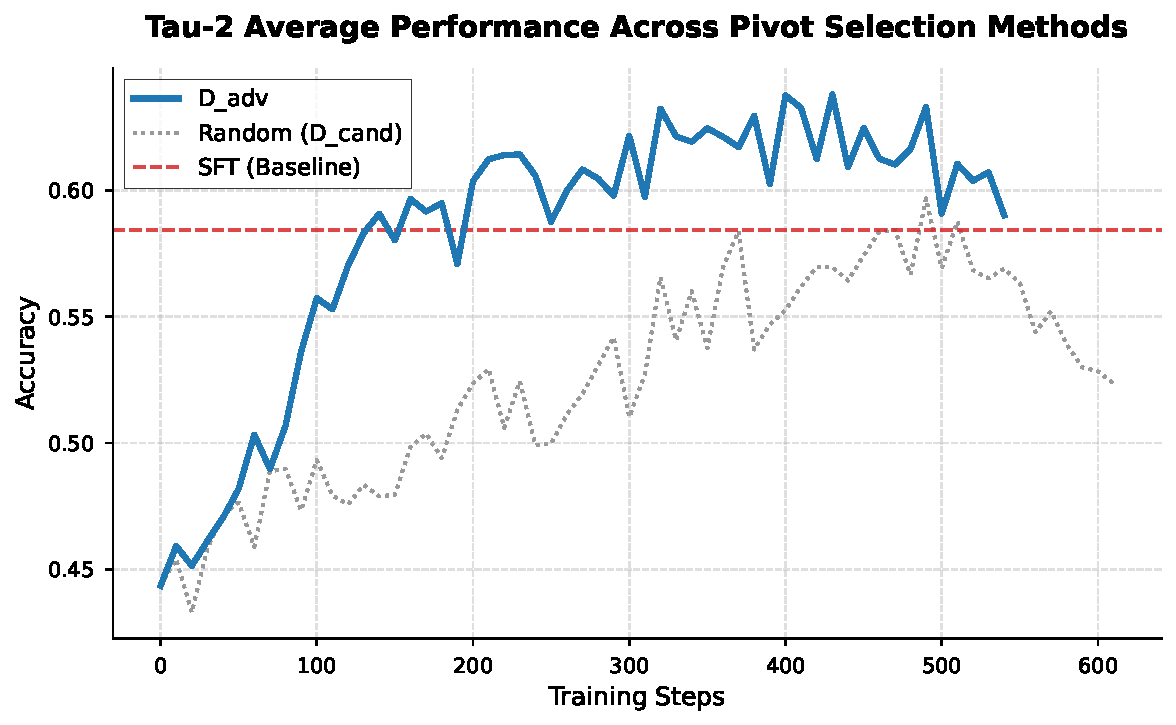
\includegraphics[width=\linewidth]{figures/main_average_validation.pdf}
        \caption{$\tau^2$-Bench accuracy over RL training. Difficult mixed-outcome pivots yield the strongest optimization and outperform same-data SFT.}
        \label{fig:tau_pivot_selection_acc}
    \end{minipage}
    \hfill
    \begin{minipage}{0.48\textwidth}
        \centering
        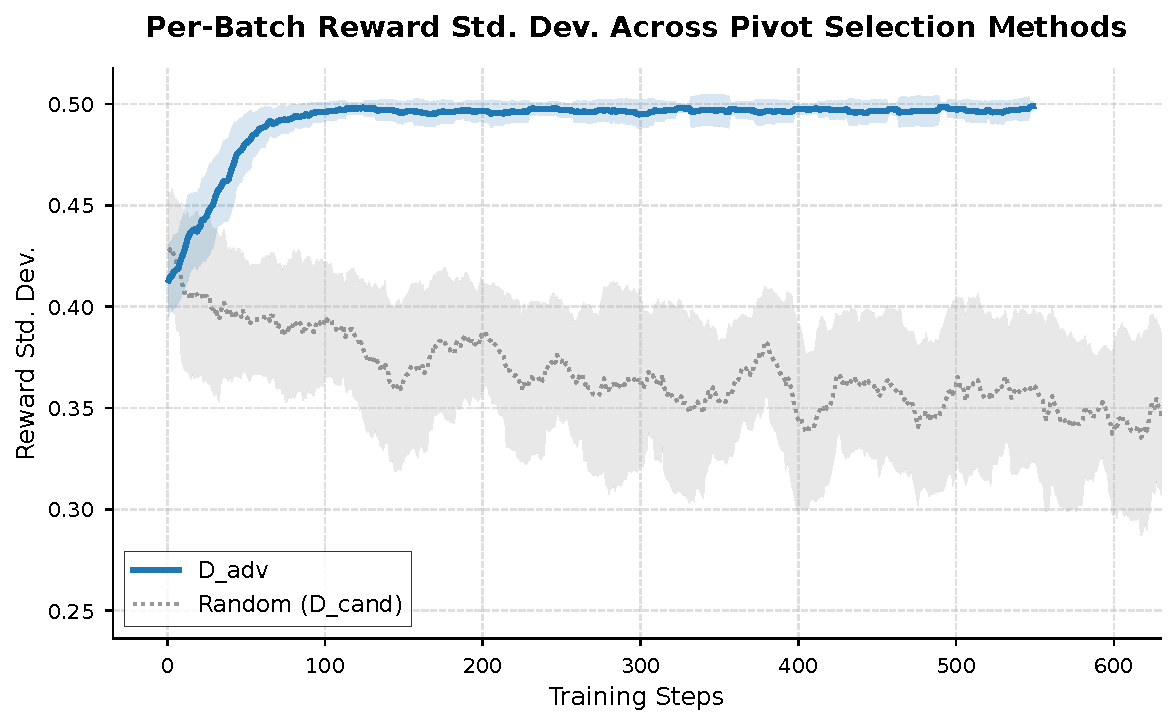
\includegraphics[width=\linewidth]{figures/tau_reward_stddev.pdf}
        \caption{$\tau^2$-Bench training reward standard deviation. More selective pivot datasets maintain higher reward variance during training.}
        \label{fig:tau_reward_std}
    \end{minipage}
\end{figure}

\begin{figure*}[t]
    \centering
    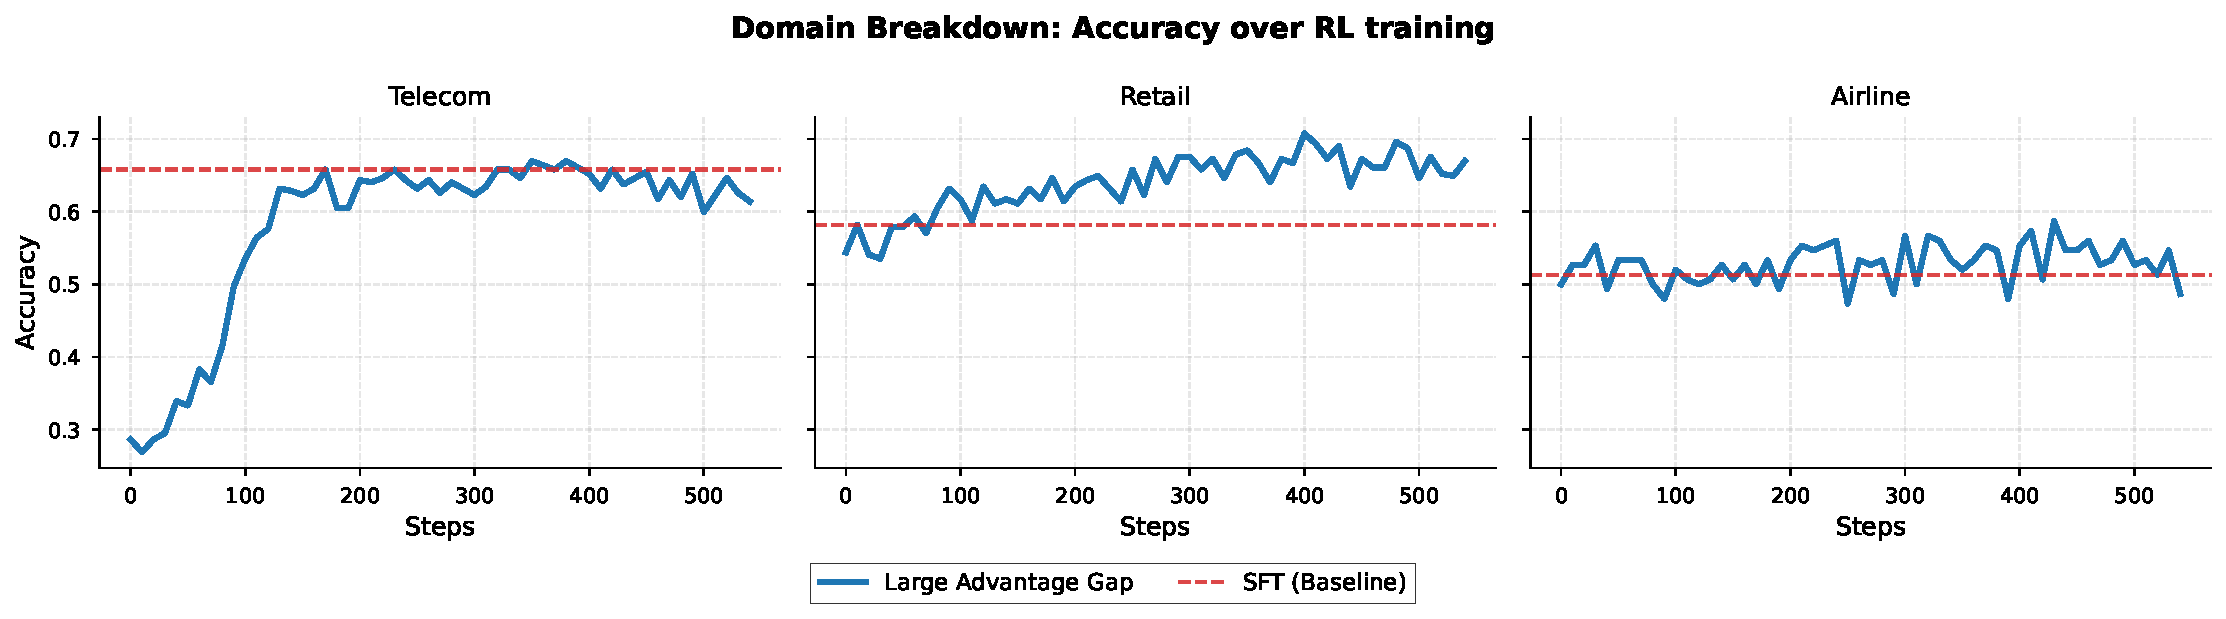
\includegraphics[width=1.0\textwidth]{figures/main_per_domain_validation_difficulty.pdf}
    \caption{Per-domain $\tau^2$-Bench accuracy over RL training for the difficult mixed-outcome pivot set. From left to right: Telecom, Retail, Airline.}
    \label{fig:tau_domain_breakdown}
\end{figure*}

Figure~\ref{fig:tau_domain_breakdown} shows the same trend broken down by domain. The strongest gains come from the difficult mixed-outcome pivot set, supporting the view that turn selection is an important part of making local RL effective.

\subsubsection{Functional reward and joint 2$\times$2 ablation}
\label{sec:joint_ablation}

We next ablate pivot selection and reward design jointly:
\[
\{\text{random pivots},\ \text{informative pivots}\}
\quad \times \quad
\{\text{strict reward},\ \text{functional reward}\}.
\]
Here, the naive local-RL baseline is \emph{random pivots + strict reward}, while full PivotRL is \emph{informative pivots + functional reward}.

\begin{table}[t]
\centering
\small
\begin{tabular}{lcc}
\toprule
\textbf{Pivot Set} & \textbf{Strict Reward} & \textbf{Functional Reward} \\
\midrule
Random pivots & [PLACEHOLDER] & [PLACEHOLDER] \\
Informative pivots & [PLACEHOLDER] & [PLACEHOLDER] \\
\bottomrule
\end{tabular}
\caption{
Joint ablation of pivot selection and reward design.
The full method corresponds to informative pivots with functional reward.
}
\label{tab:joint_component_ablation}
\end{table}

This ablation is designed to answer a simple question: are the gains coming mainly from better state selection, from a less brittle reward, or from the combination of both? Replacing strict reward with functional reward changes only the credit assignment at a fixed set of turns. Replacing random pivots with informative pivots changes only which turns are used for training. Full PivotRL combines both.

\subsection{Benchmark-specific training details}
\label{sec:benchmark_specific_details}

We now summarize the data construction and local verifiers used in each domain. Full profiling details and hyperparameters are deferred to the appendix.

\paragraph{$\tau^2$-Bench.}
We curate an SFT trajectory dataset of 281{,}774 trajectories across 838 domains using a synthetic data-generation pipeline similar to ToolAce \citep{liu2025toolacewinningpointsllm}, Kimi-K2 \citep{kimiteam2025kimik2openagentic}, and DeepSeek-V3.2 \citep{deepseekai2025deepseekv32pushingfrontieropen}. We train on top of \texttt{Qwen3-30B-A3B-Thinking-2507}. Every assistant turn is treated initially as a pivot candidate. We then evaluate random, mixed-outcome, and difficult mixed-outcome pivot sets as described in Section~\ref{sec:pivotrl_method}.

\paragraph{Terminal-Bench.}
We collect resolved trajectories from \texttt{Qwen/Qwen3-Coder-480B-A35B-Instruct} and \texttt{moonshotai/Kimi-K2-Instruct} using the Terminus-1 and Terminus-2 agents. We treat assistant bash actions as pivots and start from the difficult mixed-outcome set $\mathcal{D}_{\mathrm{adv}}$, with an additional command-deduplication step to improve diversity. The final dataset contains approximately 20{,}000 samples. The local verifier combines output-schema validation, string similarity, and equivalence-based LLM-as-judge scoring; in this setting, equivalence means that different commands can receive positive credit when they are judged to implement the same locally appropriate terminal action.

\paragraph{SWE-Bench Verified.}
We use an internal trajectory dataset generated with OpenHands \citep{wang2025openhandsopenplatformai}, OpenCode \citep{opencode}, and Codex \citep{openaicodex_software} on tasks including SWE-Gym \citep{pan2025trainingsoftwareengineeringagents} and R2E-Gym \citep{jain2025r2egymproceduralenvironmentshybrid}, using \texttt{MiniMaxAI/MiniMax-M2.5} \citep{minimax2026m25}. We evaluate mean@3 with the OpenHands harness. To construct the PivotRL dataset, we use non-error tool-call actions as pivots and filter to $\mathcal{D}_{\mathrm{adv}}$, producing a final training set of 87{,}718 samples. In the current experiments, the local verifier checks tool-call names only, so the SWE results should be interpreted as evaluating whether locally appropriate tool choice is a useful training signal rather than as a full local correctness verifier.

\paragraph{BrowseComp.}
We start from a multi-hop question-answer dataset and use an online search engine together with \texttt{DeepSeek-V3.2} to generate browsing trajectories. The final dataset contains 13{,}215 samples. The action unit in this domain is the full search-related assistant completion at a model-call boundary. Because this dataset is comparatively small, we use random filtering ($\mathcal{D}_{\mathrm{random}}$) rather than the more selective pivot sets.

\begin{table*}[t]
\centering
\small
\begin{tabular}{l c cc c}
\toprule
\multirow{2}{*}{\textbf{Benchmark}} 
& \multirow{2}{*}{\textbf{Baseline}} 
& \multicolumn{2}{c}{\textbf{Multi-Domain Training}}
& \multirow{2}{*}{\textbf{RL vs SFT ($\Delta$)}} \\
\cmidrule(lr){3-4}
& Qwen3-30B 
& \textbf{SFT} & \textbf{RL} & \\
\midrule
\midrule

\multicolumn{5}{l}{\textit{In-Domain Benchmarks}} \\
\midrule

$\tau^2$-Bench
& 44.35 
& 57.60 (+13.25) & 56.33 (+11.98) 
& -1.27 \\

SWE-Verified
& 19.07 
& [PLACEHOLDER] & 32.87 (+13.80) 
& [PLACEHOLDER] \\

Terminal-Bench
& 5.42 
& [PLACEHOLDER] & [PLACEHOLDER] 
& [PLACEHOLDER] \\

BrowseComp
& 2.50 
& [PLACEHOLDER] & [PLACEHOLDER] 
& [PLACEHOLDER] \\

\midrule
\multicolumn{5}{l}{\textit{Out-of-Domain Benchmarks}} \\
\midrule

IFBench 
& 52.04 
& 47.71 (-4.33)  & 50.41 (-1.63) 
& +2.70 \\

AIME25 
& 86.04 
& 83.13 (-2.91)  & 85.83 (-0.21) 
& +2.70 \\

MATH500 
& 98.05 
& 98.15 (+0.10)  & 98.15 (+0.10) 
& 0.00 \\

LiveCodeBench 
& 66.52 
& 60.57 (-5.95)  & 67.40 (+0.88) 
& +6.83 \\

Scicode 
& 36.83 
& 26.18 (-10.65) & 38.17 (+1.34) 
& +11.99 \\

MMLU-Pro 
& 80.84 
& 80.97 (+0.13)  & 81.14 (+0.30) 
& +0.17 \\

MMLU-ProX 
& 78.58 
& [PLACEHOLDER]  & 78.74 (+0.16) 
& [PLACEHOLDER] \\

WMT24++ 
& 36.97 
& 34.87 (-2.10)  & 36.92 (-0.05) 
& +2.05 \\

\bottomrule
\end{tabular}
\caption{
Multi-domain training results.
Only completed runs are reported.
}
\label{tab:multi_domain_results}
\end{table*}

Table~\ref{tab:multi_domain_results} extends the single-domain results to the multi-domain setting. Because several runs are still incomplete, we report only completed results and avoid over-interpreting the partially filled matrix. On the available runs, PivotRL remains competitive in-domain while preserving held-out capabilities substantially better than multi-domain SFT.

For multi-domain training, we do not summarize OOD with a single scalar in the same way as in the single-domain setting, because each policy is trained on multiple target domains simultaneously. Instead, we report held-out benchmark performance directly relative to the common base model. This makes the comparison cleaner: the reader can see where multi-domain SFT and multi-domain PivotRL differ without forcing an artificial single-domain OOD definition onto the mixed-domain case.